\apendice{Especificación de diseño}

\section{Introducción}
En cualquier proyecto la fase de diseño de las distintas partes de éste es esencial para su correcta implementación, desarrollo y evolución. En este apartado se va a comentar los distintos diseños que se han realizado para poder obtener una solución óptima, aun así hay que tener en cuenta el gran peso que tiene la investigación en este proyecto por lo que el diseño en una gran parte del proyecto no ha sido necesario.

Los diseños realizados en el proyecto han sido:
\begin{itemize}
	\item \textbf{Diseño de datos}: subapartado donde se van a mostrar las distintas estructuras de datos utilizadas, así como un conjunto de diagramas para comprender la estructura de los ficheros de ejecución del proyecto.
	\item \textbf{Diseño procedimental}: subapartado donde se va a mostrar principalmente como es la comunicación entre el flujo y las implementaciones realizadas.
\end{itemize}
\section{Diseño de datos}

Este proyecto al ser mayoritariamente un proyecto de investigación apenas tiene diseño de datos. Aun así , sí que existe un diseño donde se muestra la estructura de los ficheros necesarios para la ejecución final sobre el flujo.

Este diseño se muestra en forma de diagrama de clases, figura~\ref{fig:diacla}, donde los asteriscos en los nombres de las variables representan que realmente hay dos variables una para la parte izquierda y otra para la derecha (un ejemplo puede se el hombro*, que significa que existe un hombroI y un hombroD, los dos del mismo tipo). En el diagrama se muestra la implementación final de la posición con la clase \texttt{Posicion}, que como se comentó en el apartado~\ref{reducida}, es la versión reducida con el conjunto mínimo de cálculos necesarios.

Por otro lado, la clase \texttt{Interfaz} es la que se comunica con el flujo de datos (de ahí su nombre), en ella se carga el modelo y se crean y se comparan las posiciones.

\begin{figure}[h]
	\centering
	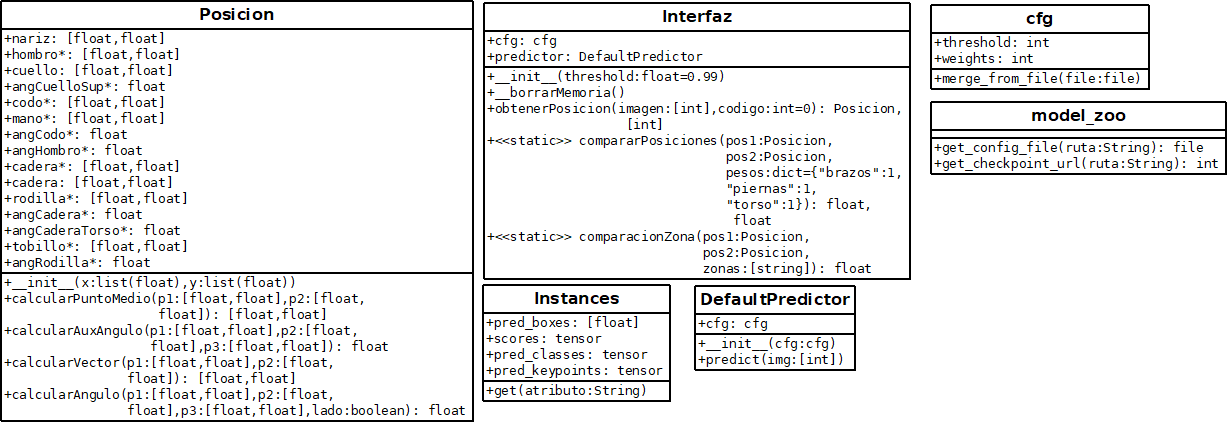
\includegraphics[width=1\textwidth]{DiagramaClaseReducido}
	\caption{Diagrama de clases.}
	\label{fig:diacla}
\end{figure}

\section{Diseño procedimental}

El diseño procedimental realizado en este proyecto, como en el caso del diseño de datos, se ha realizado sobre la implementación final en las clases que usan el flujos de datos. Estos diseño procedimentales se han realizado a partir de diagramas de secuencia, donde se muestran las dos posibbles interacciones del flujo con las clases.

En la primera posibilidad, el flujo tan solo pide las posiciones de las imágenes que va proporcionando, figura~\ref{fig:diasec1}. Como se puede ver en el diagrama de secuencias, los primero que tiene que realizar un \textit{worker} del flujo es instanciar la clase \texttt{Interfaz} donde se procede con la carga y configuración del modelo. Una vez instanciada la clase se puede hacer llamadas para obtener la estimación de la posición de un imagen (operación que se puede repetir mientras esté cargado el modelo, es decir, mientras esté vivo el \textit{worker}).

\begin{figure}[h]
	\centering
	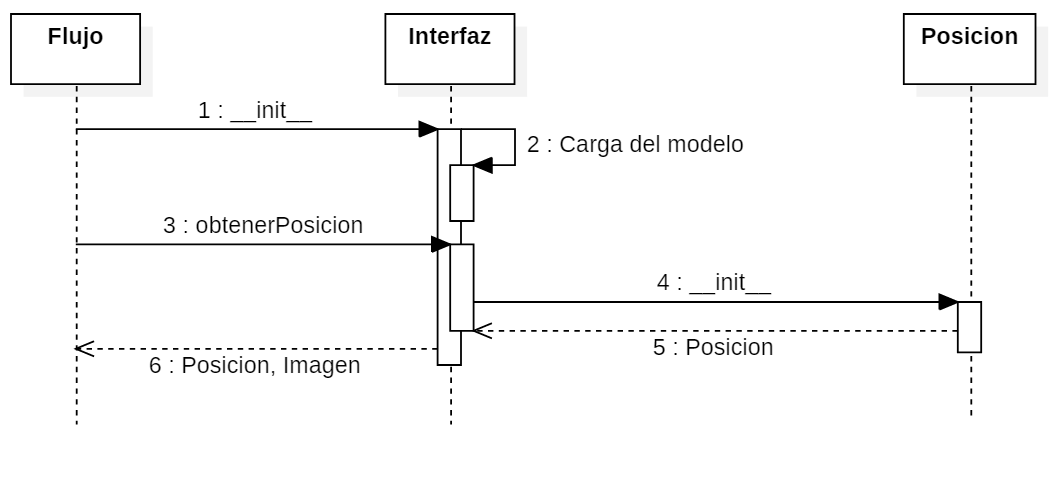
\includegraphics[width=1\textwidth]{DiagramaSecuenciaPosicion}
	\caption{Diagrama de secuencia, estimación posición.}
	\label{fig:diasec1}
\end{figure}

Por otro lado, una segunda posibilidad de la ejecución con el flujo es la comparación de posiciones, figura~\ref{fig:diasec2}. En este diagrama de secuencias se muestra como es la interacción entre los distintos elementos que trabajan con el flujo, como en el caso anterior las llamadas a la comparación y obtención de posiciones se pueden realizar mientras esté vivo el \textit{worker} que tiene el modelo cargado.

\begin{figure}[h]
	\centering
	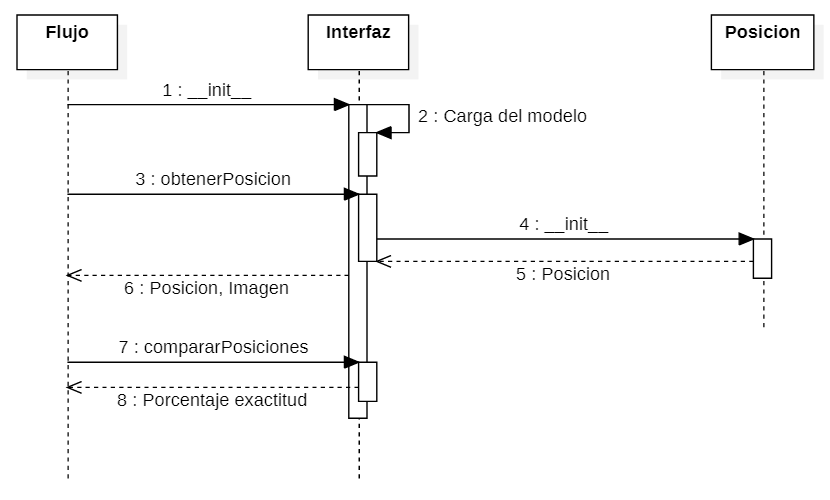
\includegraphics[width=1\textwidth]{DiagramaSecuenciaComparacion}
	\caption{Diagrama de secuencia, comparación de posiciones.}
	\label{fig:diasec2}
\end{figure}


